\documentclass[10pt]{article}
\usepackage[polish]{babel}
\usepackage[utf8]{inputenc}
\usepackage[T1]{fontenc}
\usepackage{amsmath}
\usepackage{amsfonts}
\usepackage{amssymb}
\usepackage[version=4]{mhchem}
\usepackage{stmaryrd}
\usepackage{graphicx}
\usepackage[export]{adjustbox}
\graphicspath{ {./images/} }

\begin{document}
\begin{enumerate}
  \item Znajdź wszystkie dwucyfrowe liczby, z których każda ma następującą własność: jeśli do takiej liczby dodamy liczbę utworzoną z przestawienia jej cyfr, to otrzymamy sumę, która jest kwadratem liczby naturalnej.
  \item Jaka jest najmniejsza liczba naturalna postaci \(25^{n}-11^{k}\), gdzie \(n \mathrm{i} k\) są liczbami naturalnymi różnymi od O?.
  \item Trójkąt ABC to trójkąt prostokątny o przyprostokątnych długości \(a\) i \(b\). Oblicz, w zależności od \(a\) i \(b\), sumę pól zacienionych półksiężyców.\\
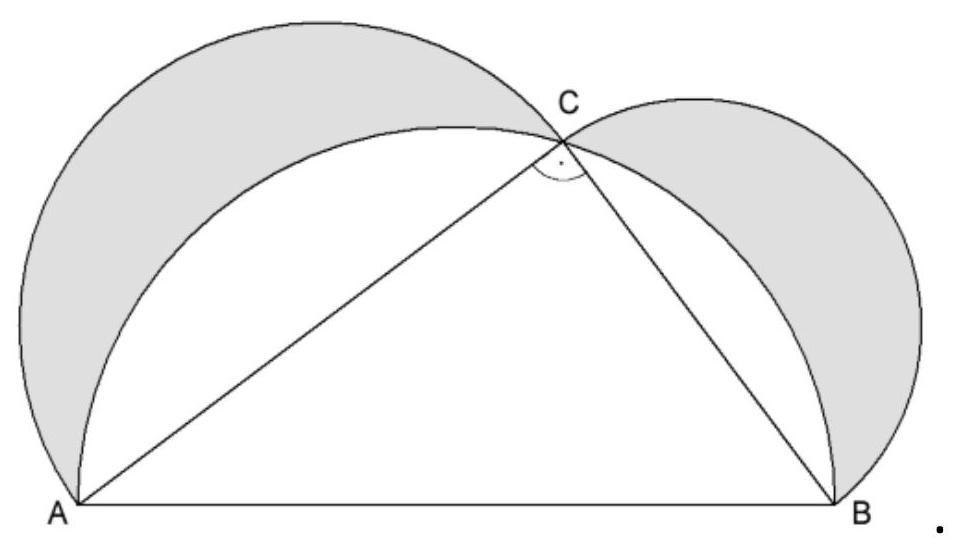
\includegraphics[max width=\textwidth, center]{2024_11_21_ae2c3732c7ed3e53a3f1g-1}
\end{enumerate}

\end{document}